\section{Fursuits are Planar Graphs}


\begin{frame}

\frametitle{\secname}

\begin{columns}
\column{0.5\textwidth}
\begin{center}
    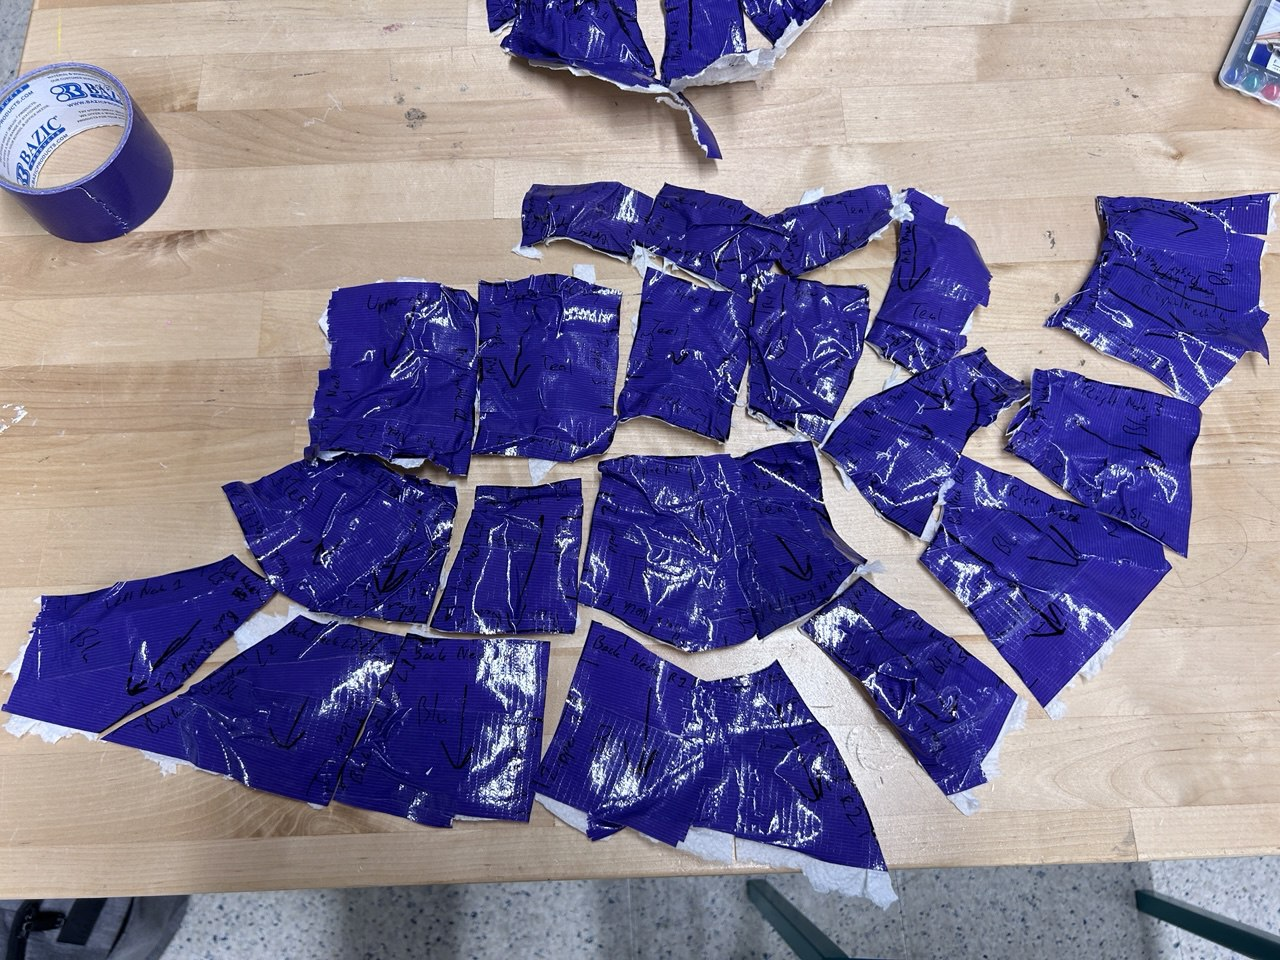
\includegraphics[scale=0.15]{slides/planar_fursuit/bunsen_furpattern.jpg}

    {
    \small 
    Bunsen's head pattern
    }
\end{center}
\column{0.5\textwidth}
\begin{center}
    \includegraphics[scale=0.048]{slides/planar_fursuit/long_furpattern.jpg}

    {
    \small
    Unsigned Long's tail pattern
    }
\end{center}

\end{columns}

\end{frame}

\begin{frame}

\frametitle{\secname}

\begin{columns}
\column{0.6\textwidth}

\begin{itemize}
\item<1-> Graph:
\begin{itemize}
\item<1-> Vertices labeled $1,2,\dots,n$
\item<1-> Edges go between two vertices
\only<1>{
\item At most $n\cdot(n-1)/2$ edges%
}%
\only<2->{
\item At most $n\cdot(n-1)/2=\emph{O(n^2)}$ edges%
}%
\footnote{Assuming simple graphs}
\end{itemize}
\item<3-> Planar graphs: graphs that can be\\drawn without crossing edges
\begin{itemize}
\item<3-> At most $3n-6=\emph{O(n)}$ edges!%
\footnote<3->{Assuming faces have degree $\ge3$}
\item<3-> Fursuits are planar graphs
\item<3-> $\text{Seam count}=O(\text{Fabric patch count})$
\end{itemize}
\end{itemize}

\column{0.4\textwidth}
\begin{figure}
\centering
\begin{tikzpicture}[every node/.style={circle,draw}]
\node (v1) {$1$};
\node (v2) [below left=of v1] {$2$};
\node (v3) [below=of v2] {$3$};
\node (v4) [below right=of v3] {$4$};
\node (v6) [below right=of v1] {$6$};
\node (v5) [below=of v6] {$5$};
\draw (v2) -- (v1) -- (v6) -- (v2) -- (v3) -- (v6) -- (v5) -- (v3) -- (v4) -- (v5);
\only<1-2>{
\draw (v1) -- (v4) (v2) -- (v5);
}
\end{tikzpicture}
\end{figure}

\end{columns}

\end{frame}